\clearpage
\section{Rossler System}
\subsection{Fixed point near the origin}
Integrating using the python script the following fixed point was found near the origin:
\begin{equation}
	x=0.007,\qquad y=-0.035, \qquad z=0.035
\end{equation}
whose jacobian eigenavlues are 
\begin{equation}
	\lambda_{1,2} = 0.1\pm i,\qquad \lambda_3 = -5.7
\end{equation}
with eignevectors
\begin{equation}
	v_1 = \mqty(1\\-0.1-i\\0.005-0.001),\qquad v_2 = \mqty(1\\-0.1+i\\0.005+0.001),\qquad v_3 = \mqty(0.17\\-0.03\\1)
\end{equation}
The two first eigenvalues produce a slow unstable spiral on the xy plane since the real part is very small but positive, and the eigenvector is mostly in the xy plane, and the third eigenvalue produces a fast strongly stable direction in z since it is strongly negative compared to the other eigenvalues and the corresponding eigenvector is strongest in the z direction.
\subsection{Varying c}
\begin{figure}[H]
	\centering
	
\includegraphics[width=0.8\textwidth]{Figure_1.png}
	\caption{Trajectories for different c values in 3D and on the xy plane.}
\end{figure}
\subsection{The chaotic attractor}
\begin{figure}[H]
	\centering
	
\includegraphics[width=0.85\textwidth]{Figure_2.png}
	\caption{x, z, and the divergence plotted over time. A red dashed line for x=c is presented and a black dashed line for div=0 is presented.}
\end{figure}
\subsubsection{Average contraction}
Calculating the average, minimum, and maximum of the divergence I found 
\begin{equation}
	\div{F}_{avg}=-5.3,\qquad \div{F}_{\min}=-14.6,\qquad \div{F}_{\max}=5.9
\end{equation}
So while the divergence is on average negative, it is not negative everywhere.
\subsubsection{The excursions from the \(z=0\) plane}
after plotting \(x(t)\) and \(z(t)\) I saw that there seems to be correlation between when x spikes and when z spikes. Looking at the equations, it's clear \(\dot{z}\) increases when \(x>c\).
\subsection{Lyapunov exponents and dimension}
\begin{figure}[H]
	\centering
	
\includegraphics[width=0.85\textwidth]{Figure_3.png}
	\caption{\(\ln\abs{\delta(t)}\) plotted over time and a fit for \(\lambda_1\).}
\end{figure}
From the fit we find \(\lambda_1=0.068\), and we were given \(\lambda_2=0\). From this initial slope we can estimate the prediction horizon as 
\begin{equation}
	T_{pred} = \frac{1}{\lambda_1}\cdot\ln\ins{\delta_{\max}/\delta_0}=269.6
\end{equation}
then we can find \(lambda_3\):
\begin{equation}
	\lambda_3 = \left<\div{\vb{F}}\right>-\lambda_1-\lambda_2=-5.313-0.067-0.0=-5.38
\end{equation}
and therefore the kaplan-yorke dimension was calcualted to be 
\begin{equation}
	D = 2.0125
\end{equation}
\subsection{Poincare section}
\begin{figure}[H]
	\centering
	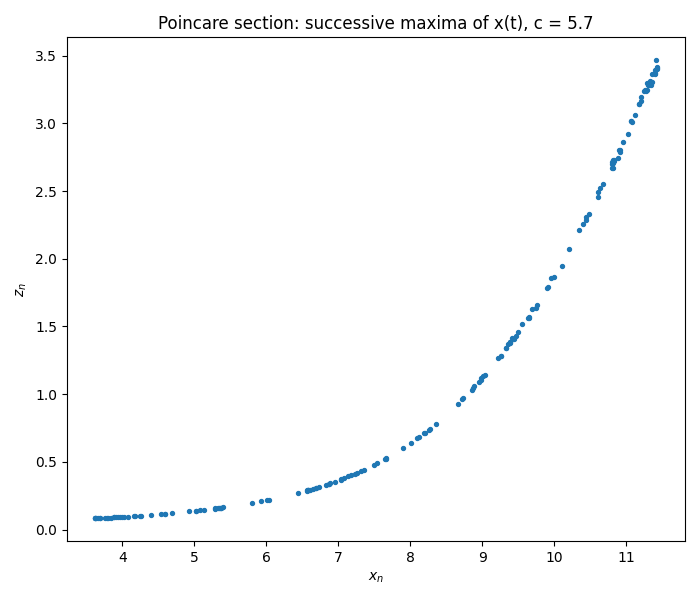
\includegraphics[width=0.85\textwidth]{Figure_4.png}
	\caption{successive maxima of x plotted in the xz plane. This fits what I expected to see, as the "holes" in the plot imply the spiky structure I saw in part c. In region beyond \(x\sim c\) we see \(z_n\) rise sharply.}
\end{figure}
\subsection{Lorenz map}
\begin{figure}[H]
	\centering
	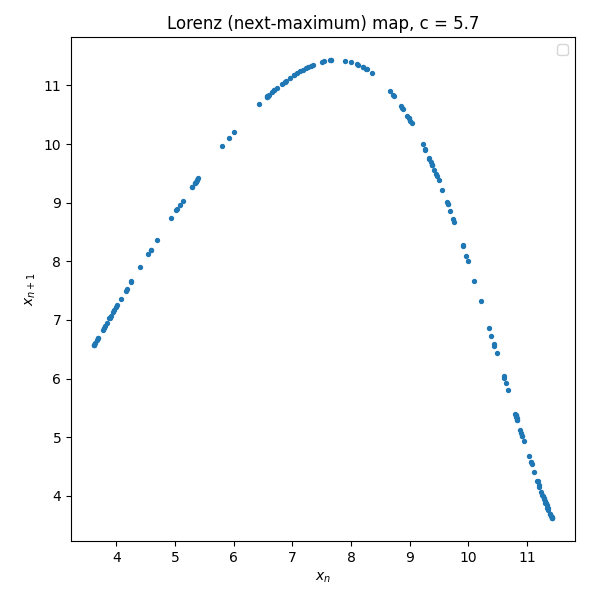
\includegraphics[width=0.85\textwidth]{Figure_5.png}
\end{figure}
which quite clearly satisfies the requirement to be a nearly one-dimensional single-humped map.